%% %%=================================================================
%% %% <UTF-8>
%% %% 北航学术论文模板使用样例
%% %% 请将以下文件与此LaTeX文件放在同一目录中.
%% %%-----------
%% %% buaa.cls              : LaTeX宏模板文件
%% %% GBT7714-2005.bst      : 国标参考文献BibTeX样式文件2005(https://github.com/Haixing-Hu/GBT7714-2005-BibTeX-Style)
%% %% GBT7714-2015.bst      : 国标参考文献BibTeX样式文件2015(https://github.com/zepinglee/gbt7714-bibtex-style)
%% %% logo-buaa.eps         : 论文封皮北航字样
%% %% head-doctor.eps       : 论文封皮北博士学术论文标题(华文行楷字体替代解决方案)
%% %% head-master.eps       : 论文封皮北学硕学术论文标题(华文行楷字体替代解决方案)
%% %% head-professional.eps : 论文封皮北专硕学术论文标题(华文行楷字体替代解决方案)
%% %% tex/*.tex             : 本模板样例中的独立章节
%% %%-----------
%% %% 请统一使用UTF-8编码.
%% %%=================================================================

%=================================================================
\documentclass[doctor,privacy,twoside]{buaa}
%=================================================================
% buaa基于ctexbook模板
% 论文样式参考自《研究生手册--二〇一五年八月》
%======================
% 模板选项:
%======================
% I.论文类型(thesis)
%--------------------
% a.学术硕士论文(master)<缺省值>
% b.专业硕士论文(professional)
% c.博士论文(doctor)
%--------------------
% II.密级(permission)
%--------------------
% a.公开(public)<缺省值>
% b.内部(privacy)
% c.秘密(secret=secret3)
% c.1.秘密3年(secret3)
% c.2.秘密5年(secret5)
% c.3.秘密10年(secret10)
% c.4.秘密永久(secret*)
% d.机密(classified=classified5)
% d.1.机密3年(classified3)
% d.2.机密5年(classified5)
% d.3.机密10年(classified10)
% d.4.机密永久(classified*)
% e.绝密(topsecret=topsecret10)
% e.1.绝密3年(topsecret3)
% e.2.绝密5年(topsecret5)
% e.3.绝密10年(topsecret10)
% e.4.绝密永久(topsecret*)
%--------------------
% III.打印设置(printtype)
%--------------------
% a.单面打印(onside)<缺省值>
% b.双面答应(twoside)
%--------------------
%=================================================================


%=================================================================
% 开启/关闭引用编号颜色:参考文献,公式,图,表,算法 等……
\refcolor{on}   % 开启: on<默认>; 关闭: off;
% 摘要和正文从右侧开始
\beginright{on} % 开启: on<默认>; 关闭: off;
% 空白页留字
\emptypagewords{[ -- This page is a preset empty page -- ]}

%=================================================================
% buaa模板已内嵌以下LaTeX工具包:
%--------------------
% ifthen, etoolbox, titletoc, remreset, remreset,
% geometry, fancyhdr, setspace, caption,
% float, graphicx, subfigure, epstopdf,
% booktabs, longtable, multirow, 
% array, enumitem
% algorithm2e, amsmath, amsthm, listings
% pifont, color, soul
%--------------------
% 请在此处添加额外工具包>> 


%=================================================================
% buaa模板已内嵌以下LaTeX宏:
%--------------------
% \highlight{text} % 黄色高亮
%--------------------
% 请在此处添加自定义宏>> 


%%=================================================================
% 论文题目及副标题-{中文}{英文}
\Title{北航博硕士学术论文\LaTeX{}模板\BUAAThesis{}}{\LaTeX{} Template of Beihang University Thesis \BUAAThesis{}}
\Subtitle{版本 \BUAAThesisVer{}}{Version \BUAAThesisVer{}}

% 学科大类,默认工学
% \Branch{工学}

% 院系,专业及研究方向
\Department{宇航学院}
\Major{控制科学与工程}
\Feild{模式识别与智能系统}

% 导师信息-{中文名}{英文名}{职称}
\Tutor{导师姓名}{Toutor}{教授}
\Cotutor{副导师姓名}{Cotutor}{高工}

% 学生姓名-{中文名}{英文名}
\Author{学生姓名}{Student}
% 学生学号
\StudentID{ID123456}

% 中图分类号
\CLC{TP391.4}

% 时间节点-{月}{日}{年}
\DateEnroll{09}{01}{2015}
\DateGraduate{03}{31}{2018}
\DateSubmit{01}{10}{2018}
\DateDefence{03}{01}{2018}

%%=================================================================
% 摘要-{中文}{英文}
\Abstract{%
  摘要是学术论文内容的简短陈述,应体现论文工作的核心思想。论文摘要应力求语言精炼准确。博士学术论文的中文摘要一般约800~1200字;硕士学位论文的中文摘要一般约500字。摘要内容应涉及本项科研工作的目的和意义、研究思想和方法、研究成果和结论。博士学位论文必须突出论文的创造性成果,硕士学位论文必须突出论文的新见解。
  
  关键字是为用户查找文献,从文中选取出来揭示全文主体内容的一组词语或术语,应尽量采用词表中的规范词(参考相应的技术术语标准)。关键词一般3~5个,按词条的外延层次排列(外延大的排在前面)。关键词之间用逗号分开,最后一个关键词后不打标点符号。
  
  为了国际交流的需要,论文必须有英文摘要。英文摘要的内容及关键词应与中文摘要及关键词一致,要符合英语语法,语句通顺,文字流畅。英文和汉语拼音一律为Times New Roman体,字号与中文摘要相同。
  }{%
  What were you doing 500 years ago? Oh, that’s right nothing, because you didn’t exist yet. In fact, several generations of your family had yet to leave their mark on the world, but one very special shark may already have been swimming in the chilly North Atlantic at that time, and the incredible animal is somehow still alive today.
  
  Scientists studying Greenland sharks observed the particularly old specimen just recently, and after studying it they’ve determined that the creature is approximately 272 to 512 years old. That’s an absolutely insane figure, and if its age lands towards the higher end, it makes the animal the oldest observed living vertebrate on the entire planet.
  
  Greenland sharks are an incredible species in a number of ways, but most notable is its longevity. The sharks are well over 100 years old before even reaching sexual maturity, and regularly live for centuries. This particularly old specimen, along with 27 others, were analyzed using radiocarbon dating. The reading came back at around 392 years, but potential margin of error means the animal’s true age is somewhere between 272 and 512.
  
  The shark, which is a female, measures an impressive 18 feet long. That’s pretty large, but it might not sound particularly large for an ocean-dwelling creature that lives hundreds of years. That is, until you consider that the Greenland shark only grows around one centimeter per year. With that in mind, 18 feet is actually downright massive.
  
  As for how this particular shark species manages to live so incredibly long, scientists attribute a lot of its longevity to its sluggish metabolism, as well as its environment. The frigid waters where the sharks thrive is thought to increase overall lifespan in a variety of ways. Past research has shown that cold environments can help slow aging, and these centuries-old sharks are most certainly benefiting from their chilly surroundings.
  
  --- Online news {\it Scientists find incredible shark that may be over 500 years old and still kicking\/}, 12.16.2017. (http://bgr.com/2017/12/14/oldest-shark-greenland-512-years-old/).
}
% 关键字-{中文}{英文}
\Keyword{%
    北航,学术论文,博士,硕士,专业硕士,中文,\LaTeX{}模板,\BUAAThesis{}
  }{%
    News, BGR, Shark
}

% 图标目录
\Listfigtab{on} % 启用: on<默认>; 关闭: off;

% 缩写定义 按tabular环境或其他列表环境编写
\Abbreviations{ \centering
\begin{tabular}{cl}
  $E$ & 能量 \\
  $m$ & 质量 \\
  $c$ & 光速 \\
  $P$ & 概率 \\
  $T$ & 时间 \\
  $v$ & 速度 \\
\end{tabular}
}

\begin{document}

%%=================================================================
% 标题级别
%--------------------
% \chapter{第一章}
% \section{1.1 小节}
% \subsection{1.1.1 条}
% \subsubsection{1.1.1.1}
% \paragraph{1.1.1.1.1}
% \subparagraph{1.1.1.1.1.1}
%--------------------
%%=================================================================

% 绪论
% [绪论]
% 此次为本LaTeX模板的简介
\chapter{绪论}

大家好,这是北航论文\LaTeX{}模板(\CTeX{}-Based)---\BUAAThesis{}。

\BUAAThesis{}为北航研究生学位论文模板,适用于理工类博士、学术硕士和专业硕士。本\LaTeX{}模板参考自2015年8月版北航《研究生手册》(以下简称《手册》),具体要求请参见各自的《手册》,最终成文格式需参考学院要求及打印方意见。本模板中大量内容和说明直接摘抄自《手册》(2015年8月版),基本覆盖了论文内容和格式方面的要求。Mac系统下请采用\verb|buaa_mac|宏包并使用XeLaTeX编译。

文献著录BibTeX样式采用Haixing Hu开源的2005版参考文献著录BibTeX样式\href{https://github.com/Haixing-Hu/GBT7714-2005-BibTeX-Style}{GBT~7714-2005}及Zeping Lee开源的2015版参考文献著录BibTeX样式\href{https://github.com/zepinglee/gbt7714-bibtex-style}{GBT7714-2015},在此感谢两位的开源分享。请自行选用:\\
\verb|\Bib{GBT7714-2005}{yourRefFile}|或\\
\verb|\Bib{GBT7714-2015}{yourRefFile}|。


本模板已上传GitHub\footnote{\href{https://github.com/CheckBoxStudio/BUAAThesis}{https://github.com/CheckBoxStudio/BUAAThesis}},该仓库中同时也包含了相应的Word模板。

意见及问题反馈请联系:\\
\indent E-mail:weiqm@buaa.edu.cn\\
\indent GitHub:\href{https://github.com/CheckBoxStudio/BUAAThesis/issues}{https://github.com/CheckBoxStudio/BUAAThesis/issues}

%%============================
\section{概述}
学位论文是标明作者从事科学研究取得的创造性成果和创新见解,并以此为内容撰写的、作为申请学位时评审用的学位论文。

硕士学位论文应该表明作者在本门学科上掌握了坚实的基础理论和系统的专门知识,对所研究的课题有新的见解,并具有从事科学研究工作或独立担任专门技术工作能力。

博士学位论文应表明作者在本门学科上掌握了坚实广阔的基础理论和系统深入的专门知识,在科学和专门技术上做出了创造性的成果,并具有独立从事科学研究工作能力。

%%============================
\section{内容要求}
论文应立论正确、推理严谨、说明透彻、数据可靠。

论文应结构合理、层次分明、叙述准确、文字简练、文图规范。对于涉及作者创新性工作和研究特点的内容应重点论述,做到数据或实例丰富、分析全面深入。文中引用的文献资料必须表明来源,使用的计量单位、绘图规范应符合国家标准。

论文内容包括:选题的背景、依据及意义;文献及相关研究综述、研究及设计方案、实验方法、装置和实验结果;理论的证明、分析和结论;重要的计算、数据、图表、曲线及相关分析;必要的附录、相关的参考文献目录等,如表\ref{tab:papercomponents}。

\centerline{-----------$\downarrow$-----------Space Check-----------$\downarrow$-----------}
\begin{table}[h]
  \caption{学位论文组成}
  \label{tab:papercomponents}
  \centering
  \begin{tabular}{cp{16\ccwd}p{4cm}}
    \toprule
    {\bfseries 装订顺序} & \multicolumn{1}{c} {\bfseries 内容} & \multicolumn{1}{c} {\bfseries 说明}  \\
    \midrule
    1 & 封面(中、英文)& \\
    2 & 题名页          & \\
    3 & 独创性声明和使用授权书 & \\
    4 & 中文摘要        & \\
    5 & 英文摘要        & \\
    6 & 目录            & \\
    7 & 图表清单及主要符号表  & 根据具体情况可省略 \\
    8 & 主体部分        & \\
    9 & 参考文献        & \\
    10& 附录            & \\
    11&攻读博士学位期间取得的研究成果/ 攻读硕士学位期间取得的学术成果 & 注意博士的是研究成果,硕士的是学术成果 \\
    12& 致谢            & \\
    13& 作者简洁        & 硕士学位论文无此项 \\
    \bottomrule
  \end{tabular}
\end{table}
\centerline{-----------$\uparrow$-----------Space Check-----------$\uparrow$-----------}

%%----------------------
\subsection{封面}
\label{sec:error1}

{\bfseries 中图分类号}:根据论文主题内容对照《中国图书分类法》选取;

{\bfseries 论文编号}:北航单位代码(10006)+学号;

{\bfseries 密级}:保密审批通过论文需在封面、题名页直接把相应的“密级☆”及“保密期限”表注在右上角(非密论文务必将相应内容清除),并将《涉密论文审批通知》复印件附在论文最后。密级按由低到高可分为“秘密”、“机密”、“绝密”三级,保密期限可分为“3年”、“5年”、“10年”、“永久”,例如“密级☆ 5年”。鼓励尽量对学位论文进行去密处理;

{\bfseries 学科专业}:以国务院学位委员会批准的授予博士、硕士学位和培养研究生的学科、专业目录中的学科专业为准,一般为二级学科。对专业学位应填相应的工程领域(如航空工程)或专业学位(工商管理硕士)名称;

{\bfseries 指导教师}:以研究生院批准招生的为准,一般只能写一名指导老师,如有经主管部门批准的副指导教师或联合指导老师,可增1名指导教师;

{\bfseries 培养院系}:应准确填写培养的学院或独立系的全称。

%%----------------------
\subsection{题名页}

{\bfseries 研究方向}:只填写一个,应比学科专业的二级学科更具体,但比论文关键词的覆盖面更广,一般为学科分类号对应的研究方向;

{\bfseries 申请学位级别}:学科门类+学位,学科门类有哲学、经济学、法学、教育学、文学、历史学、理学、工学、农学、医学、军事学和管理学等12个学科门类以及专业学位类别(工程、工程管理、公共行政管理、软件工程);

{\bfseries 工作完成日期}:包括学习日期(从研究生入学至毕业时间)、论文提交日期(论文送审评阅时间)、论文答辩日期、学位授予日期;除学位授予日期可以不填外,其他均需准确填写,一律用阿拉伯数字填写日期;

{\bfseries 学位授予单位}:北京航空航天大学。

%%----------------------
\subsection{独创性声明和使用授权书}

必须由作者、指导教师亲笔签名并填写日期。

%%----------------------
\subsection{摘要}

中文摘要包括“摘要”字样,摘要正文及关键词。对于中英文摘要,都必须在摘要的最下方另起一行。

摘要是学位论文内容的简短陈述,应体现论文工作的核心思想。论文摘要应力求语言精炼准确。博士学位论文的中文摘要一般约800$\sim$1200字;硕士学位论文的中文摘要一般约500字。摘要内容应涉及本项科研工作的目的和意义、研究思想和方法、研究成果和结论。博士学位论文必须突出论文的创造性成果,硕士学位论文必须突出论文的新见解。

关键字是为用户查找文献,从文中选取出来揭示全文主体内容的一组词语或术语,应尽量采用词表中的规范词(参考相应的技术术语标准)。关键词一般3$\sim$5个,按词条的外延层次排列(外延大的排在前面)。关键词之间用逗号分开,最后一个关键词后不打标点符号。

为了国际交流的需要,论文必须有英文摘要。英文摘要的内容及关键词应与中文摘要及关键词一致,要符合英语语法,语句通顺,文字流畅。英文和汉语拼音一律为Times New Roman体,字号与中文摘要相同。

%%----------------------
\subsection{目录}

目录按章、节、条和标题编写,一般为二级或三级,目录中应包括绪论(或引言)、论文主体章节、结论、附录、参考文献、附录、攻读学位期间取得的成果等。

%%----------------------
\subsection{图表清单及主要符号表}

如果论文中图表较多,可以分别列出清单置于目录之后。图的清单应有序号、图题和页码,表的清单应有序号、标题和页码。
全文中常用的符号、标志、缩略词、首字母缩写、计量单位、名词、术语等的注释说明,如需汇集,可集中在图和表清单后的主要符号表中列出,符号表排列顺序按英文及其相关文字顺序排出。

%%----------------------
\subsection{主体部分}

一般应包括:绪论(或引言)、正文、结论等部分。

每章应另起一页。章节标题不得使用标点符号,尽量不采用英文缩写词,对必须采用者,应使用本行业的通用缩写词。
三级标题的层次对理工类建议按章(如“第一章”)、节(如“1.1”)、条(如“1.1.1”)的格式编写;对社科、文学类建议按章(如“一、”)、节(如“(一)”)、条(如“1、”)的格式编写,各章题序的阿拉伯数字用Times New Roman字体。

博士学位论文一般为6$\sim$10万字,硕士学位论文一般为3$\sim$5万字。

%%----------------------
\subsection{参考文献}

学术研究应精确、有据、坦诚、创新、积累。而其中精确、有据和积累需要建立在正确对待前人学术成果的基础上。凡有直接引用他人成果之处,均应加标注说明列于参考文献中,以避免论文抄袭现象的发生。

研究生论文参考文献著录及标引按照国家标准《文后参考文献著录规则》(GB774)和中国博硕士学位论文编写与交换格式。

%%----------------------
\subsection{符录}

附录作为论文主体的补充项目,并不是必需的。

%%----------------------
\subsection{成果}

对于博士学位论文,名称用“攻读博士学位期间取得的研究成果”,一般包括:

攻读博士学位期间取得的学术成果:攻读博士学位期间取得的学术成果:列出攻读博士期间发表(含录用)的与学位论文相关的学位论文、发表专利、著作、获奖项目等,书写格式与参考文献格式相同;

攻读博士期间参与的主要科研项目:列出攻读博士学位期间参与的与学位论文相关的主要科研项目,包括项目名称,项目来源,研制时间,本人承担的主要工作。

对于硕士学位论文,名称用“攻读硕士学位期间取得的学术成果”,只列出攻读硕士学位期间发表(含录用)的与学位论文相关的学位论文、发表专利、著作、获奖项目等,书写格式与参考文献格式相同。

%%----------------------
\subsection{致谢}
致谢中主要感谢指导教师在和学术方面对论文的完成有直接贡献及重要帮助的团体和人士,以及感谢给予转载和引用权的资料、图片、文献、研究思想和设想的所有者。致谢中还可以感谢提供研究经费及实验装置的基金会或企业等单位和人士。致谢辞应谦虚诚恳,实事求是,切记浮夸与庸俗之词。

%%----------------------
\subsection{作者简介}

博士学位论文应该提供作者简介,主要包括:姓名、性别、出生年月日、民族、出生的;简要学历、工作经历(职务);以及攻读博士学位期间获得的其他奖项(除攻读学位期间取得的研究成果之外)。



% 说明
% 本LaTeX模板的一般使用说明
\chapter{说明}

Again,这是北航论文\LaTeX{}模板(\CTeX{}-Based)\BUAAThesis{}。

本\LaTeX{}模板为北航研究生学位论文模板,适用于理工类博士、学术硕士和专业硕士。本\LaTeX{}模板参考自2015年8月版北航《研究生手册》,具体要求请参见各自的《手册》,最终成文格式需参考学院要求及打印方意见。本模板中大量内容和说明直接摘抄自《手册》(2015年8月版),基本覆盖了论文内容和格式方面的要求。

本模板已上传\href{https://github.com/CheckBoxStudio/BUAAThesis}{GitHub},该仓库中同时也包含了相应的Word模板。

%-----------------------------
\section{宏包使用}

请将以下文件与此LaTeX文件放在同一目录中:

\begin{tabular}{ll}
 \verb|buaa.cls |             & $\triangleright$ LaTeX宏模板文件 \\
 \verb|buaa_mac.cls |         & $\triangleright$ LaTeX宏模板文件(For Mac with XeLaTeX) \\
 \verb|GBT7714-2005.bst|      & $\triangleright$ 国标参考文献BibTeX样式文件2005 \\
 \verb|GBT7714-2015.bst|      & $\triangleright$ 国标参考文献BibTeX样式文件2015 \\
 \verb|logo-buaa.eps|         & $\triangleright$ 论文封皮北航字样 \\
 \verb|head-doctor.eps|       & $\triangleright$ 论文封皮北博士学位论文标题\\
 \verb|head-master.eps|       & $\triangleright$ 论文封皮北学硕学位论文标题 \\
 \verb|head-professional.eps| & $\triangleright$ 论文封皮北专硕学位论文标题\\
 \verb|tex/*.tex|             & $\triangleright$ 本模板样例中的独立章节\\
\end{tabular}\\

通过 \verb|\documentclass[<thesis>,<permission>,<printtype>,<ctexbookoptions>]{buaa}|载入宏包:
\begin{itemize}[leftmargin=3cm]
  \item[{\tt thesis} $\triangleright$]  论文类型(thesis),可选值:\\
    a) 学术硕士论文(\verb|master|)[缺省值]\\
    b) 专业硕士论文(\verb|professional|)\\
    c) 博士论文(\verb|doctor|)
  \item[{\tt permission} $\triangleright$] 密级(permission),可选值: \\
    a) 公开(\verb|public|)[缺省值]\\
    b) 内部(\verb|privacy|)\\
    c) 秘密(\verb|secret|=\verb|secret3|)\\
    --- c.1) 秘密3年(\verb|secret3|)\\
    --- c.2) 秘密5年(\verb|secret5|)\\
    --- c.3) 秘密10年(\verb|secret10|)\\
    --- c.4) 秘密永久(\verb|secret*|)\\
    d) 机密(\verb|classified|=\verb|classified5|)\\
    --- d.1) 机密3年(\verb|classified3|)\\
    --- d.2) 机密5年(\verb|classified5|)\\
    --- d.3) 机密10年(\verb|classified10|)\\
    --- d.4) 机密永久(\verb|classified*|)\\
    e) 绝密(\verb|topsecret|=\verb|topsecret10|)\\
    --- e.1) 绝密3年(\verb|topsecret3|)\\
    --- e.2) 绝密5年(\verb|topsecret5|)\\
    --- e.3) 绝密10年(\verb|topsecret10|)\\
    --- e.4) 绝密永久(\verb|topsecret*|)
  \item[{\tt printtype} $\triangleright$] 打印属性(printtype),可选值: \\
    a) 单面打印(\verb|onside|)[缺省值]\\
    b) 双面打印(\verb|twoside|)\\
  \item[{\tt ctexbookoptions} $\triangleright$] 其他选项将被传递给{\tt ctexbook}文档类。\\
  一种使用场景为:
  CTeX在Linux下默认使用Fandol字体,受字体所限,某些生僻字(如姓名)无法显示。
  一种解决办法为自行在系统中安装CTeX所需的字体,如方正字体。
  使用{\tt ctexbookoptions}机制,将{\tt fontset=founder}加入到{\tt buaa}文档类的选项中可避免生僻字乱码的问题。
\end{itemize}

模板已内嵌LaTeX工具包: 
 {\tt ifthen},{\tt etoolbox},{\tt titletoc},{\tt remreset},{\tt remreset}, 
 {\tt geometry},{\tt fancyhdr},{\tt setspace},{\tt caption},{\tt float}, 
 {\tt graphicx},{\tt subfigure},{\tt epstopdf},
 {\tt book\-tabs},{\tt longtable},{\tt multirow},{\tt array}, {\tt enumitem}, 
 {\tt algorithm2e},{\tt amsmath},{\tt amsthm},{\tt listings},
 {\tt pifont},{\tt color},{\tt soul}, {\tt newtxtext}, {\tt newtxmath}。

模板已内嵌宏:\verb|\highlight{text}|(黄色高亮)。

请统一使用UTF-8编码。



%-----------------------------
\section{选项设置}

\begin{itemize}[leftmargin=3cm]
  \item[{\tt  $\backslash$refcolor} $\triangleright$]  开启/关闭引用编号颜色,包括参考文献,公式,图,表,算法等\\
  \texttt{on}:开启 [默认]\\
  \texttt{off}:关闭
  \item[{\tt $\backslash$beginright} $\triangleright$]  摘要和正文从右侧开始\\
  \texttt{on}:开启 [默认]\\
  \texttt{off}:关闭
  \item[{\tt $\backslash$emptypageword} $\triangleright$]  空白页留字
  \item[{\tt $\backslash$Listfigtab} $\triangleright$]  是否使用图标清单目录\\
  \texttt{on}:开启 [默认]\\
  \texttt{off}:关闭
\end{itemize}


%-----------------------------
\section{章节撰写}
本模板支持以下标题级别标题级别:

\begin{tabular}{ll}
  \verb|\chapter{章}|              & $\triangleright$ 第一章 \\
  \verb|\chapter*{无章号章}|       & $\triangleright$ 无章号章 \\
  \verb|\chaptera{无章号有目录章}| & $\triangleright$ 无章号有目录章 \\
  \verb|\summary|                  & $\triangleright$ 总结\\
  \verb|\appendix|                 & $\triangleright$ 附录\\
  \verb|\achievement|              & $\triangleright$ 攻读学位期间取得的成果\\
  \verb|\acknowledgments|          & $\triangleright$ 致谢\\
  \verb|\biography|                & $\triangleright$ 作者简介\\
  \verb|\section{节}|              & $\triangleright$ 1.1 节\\
  \verb|\subsection{条}|           & $\triangleright$ 1.1.1 条\\
  \verb|\subsubsection{A}|         & $\triangleright$ 1.1.1.1 A\\
  \verb|\paragraph{a}|             & $\triangleright$ 1.1.1.1.1 a\\
  \verb|\subparagraph{a)}|         & $\triangleright$ 1.1.1.1.1.1 a)\\
\end{tabular}

%-----------------------------
\section{注意事项}
\begin{itemize}
  \item[$\triangleright$] \textit{中文斜体}将转换为楷体;
  \item[$\triangleright$] \textbf{中文粗体}正常;
  \item[$\triangleright$] 英文粗体\textbf{English}、斜体\textit{English}均正常;
  \item[$\triangleright$] 中文标点的断行效果不好;
  \item[$\triangleright$] \verb|\label{<text>}|中不能使用中文;
  \item[$\triangleright$] 浮动体与正文之间的距离是弹性的;
  \item[$\triangleright$] 命令符与汉字之间请注意加空格以避免undefined错误(pdfLaTeX下好像一般不存在这个问题,主要在XeLaTeX编译环境下发生);
\end{itemize}

%-----------------------------
\section{ToDo}
\begin{itemize}
  \item[$\triangleright$] 数学环境的行间隔;
  \item[$\triangleright$] 参考文献的行间隔;
\end{itemize}

%-----------------------------
\section{意见及问题反馈}

\indent E-mail:weiqm@buaa.edu.cn

\indent GitHub:\href{https://github.com/CheckBoxStudio/BUAAThesis/issues}{https://github.com/CheckBoxStudio/BUAAThesis/issues}


% 示例
% 本LaTeX模板的使用示例
\chapter{示例}

%==============================
\section{参考文献引用}

%--------------------------------
\subsection{数字标注}
\noindent
\begin{tabular}{l@{\quad$\Rightarrow$\quad}l}
  \verb|\cite{knuth86a}| & \cite{knuth86a}\\
  \verb|\citet{knuth86a}| & \citet{knuth86a}\\
  \verb|\citet[chap.~2]{knuth86a}| & \citet[chap.~2]{knuth86a}\\[0.5ex]
  \verb|\citep{knuth86a}| & \citep{knuth86a}\\
  \verb|\citep[chap.~2]{knuth86a}| & \citep[chap.~2]{knuth86a}\\
  \verb|\citep[see][]{knuth86a}| & \citep[see][]{knuth86a}\\
  \verb|\citep[see][chap.~2]{knuth86a}| & \citep[see][chap.~2]{knuth86a}\\[0.5ex]
  \verb|\citet*{knuth86a}| & \citet*{knuth86a}\\
  \verb|\citep*{knuth86a}| & \citep*{knuth86a}\\
\end{tabular}
\par\noindent
\begin{tabular}{l@{\quad$\Rightarrow$\quad}l}
  \verb|\citet{knuth86a,tlc2}| & \citet{knuth86a,tlc2}\\
  \verb|\citep{knuth86a,tlc2}| & \citep{knuth86a,tlc2}\\
  \verb|\cite{knuth86a,knuth84}| & \cite{knuth86a,knuth84}\\
  \verb|\upcite{knuth86a,knuth84}| & \upcite{knuth86a,knuth84}\\
  \verb|\citet{knuth86a,knuth84}| & \citet{knuth86a,knuth84}\\
  \verb|\citep{knuth86a,knuth84}| & \citep{knuth86a,knuth84}\\
  \verb|\cite{knuth86a,knuth84,tlc2}| & \cite{knuth86a,knuth84,tlc2}\\
\end{tabular}

%--------------------------------
\subsection{数字标注-上标形式}
\noindent
\begin{tabular}{l@{\quad$\Rightarrow$\quad}l}
  \verb|\upcite{knuth86a}| & \upcite{knuth86a}\\
  \verb|\upcite{knuth86a,knuth84,tlc2}| & \upcite{knuth86a,knuth84,tlc2}\\
\end{tabular}
\par\noindent
实现源码:\verb|\newcommand{\upcite}[1]{\textsuperscript{\cite{#1}}}|。


%--------------------------------
\subsection{著者-出版年制标}
\citestyle{authoryear}
\noindent
\begin{tabular}{l@{\quad$\Rightarrow$\quad}l}
  \verb|\cite{knuth86a}| & \cite{knuth86a}\\
  \verb|\citet{knuth86a}| & \citet{knuth86a}\\
  \verb|\citet[chap.~2]{knuth86a}| & \citet[chap.~2]{knuth86a}\\[0.5ex]
  \verb|\citep{knuth86a}| & \citep{knuth86a}\\
  \verb|\citep[chap.~2]{knuth86a}| & \citep[chap.~2]{knuth86a}\\
  \verb|\citep[see][]{knuth86a}| & \citep[see][]{knuth86a}\\
  \verb|\citep[see][chap.~2]{knuth86a}| & \citep[see][chap.~2]{knuth86a}\\[0.5ex]
  \verb|\citet*{knuth86a}| & \citet*{knuth86a}\\
  \verb|\citep*{knuth86a}| & \citep*{knuth86a}\\
\end{tabular}
\par\noindent
\begin{tabular}{l@{\quad$\Rightarrow$\quad}l}
  \verb|\citet{knuth86a,tlc2}| & \citet{knuth86a,tlc2}\\
  \verb|\citep{knuth86a,tlc2}| & \citep{knuth86a,tlc2}\\
  \verb|\cite{knuth86a,knuth84}| & \cite{knuth86a,knuth84}\\
  \verb|\citet{knuth86a,knuth84}| & \citet{knuth86a,knuth84}\\
  \verb|\citep{knuth86a,knuth84}| & \citep{knuth86a,knuth84}\\
\end{tabular}
\citestyle{numbers}

%--------------------------------
\subsection{其他形式的标注}
\noindent
\begin{tabular}{l@{\quad$\Rightarrow$\quad}l}
  \verb|\citealt{tlc2}| & \citealt{tlc2}\\
  \verb|\citealt*{tlc2}| & \citealt*{tlc2}\\
  \verb|\citealp{tlc2}| & \citealp{tlc2}\\
  \verb|\citealp*{tlc2}| & \citealp*{tlc2}\\
  \verb|\citealp{tlc2,knuth86a}| & \citealp{tlc2,knuth86a}\\
  \verb|\citealp[pg.~32]{tlc2}| & \citealp[pg.~32]{tlc2}\\
  \verb|\citenum{tlc2}| & \citenum{tlc2}\\
  \verb|\citetext{priv.\ comm.}| & \citetext{priv.\ comm.}\\
\end{tabular}

\noindent
\begin{tabular}{l@{\quad$\Rightarrow$\quad}l}
  \verb|\citeauthor{tlc2}| & \citeauthor{tlc2}\\
  \verb|\citeauthor*{tlc2}| & \citeauthor*{tlc2}\\
  \verb|\citeyear{tlc2}| & \citeyear{tlc2}\\
  \verb|\citeyearpar{tlc2}| & \citeyearpar{tlc2}\\
\end{tabular}

\section{浮动体}

\section{算法环境}

模板中使用 \texttt{algorithm2e} 宏包实现算法环境。关于该宏包的具体用法请阅读宏包的官方文档。\\
\centerline{-----------$\downarrow$-----------Space Check-----------$\downarrow$-----------}

\begin{algorithm}[!h]
  %\SetAlgoLined
  %\SetAlgoVlined
  \caption{A How to (plain).}
  \KwData{this text}
  \KwResult{how to write algorithm with \LaTeX2e{} }
  
  initialization\;
  \While{not at end of this document}{
    read current\;
    \eIf{understand}{
      go to next section\;
      current section becomes this one\;
    }{
      go back to the beginning of current section\;
    }
  }
\end{algorithm}

\centerline{-----------$\uparrow$-----------Space Check-----------$\uparrow$-----------}

\RestyleAlgo{ruled}
\begin{algorithm}[!h]
  \caption{A How to (ruled).}
  \KwData{this text}
  \KwResult{how to write algorithm with \LaTeX2e{} }
  
  initialization\;
  \While{not at end of this document}{
    read current\;
    \eIf{understand}{
      go to next section\;
      current section becomes this one\;
    }{
      go back to the beginning of current section\;
    }
  }
\end{algorithm}

\RestyleAlgo{boxed}
\begin{algorithm}[!h]
  \caption{A How to (boxed).}
  \KwData{this text}
  \KwResult{how to write algorithm with \LaTeX2e{} }
  
  initialization\;
  \While{not at end of this document}{
    read current\;
    \eIf{understand}{
      go to next section\;
      current section becomes this one\;
    }{
      go back to the beginning of current section\;
    }
  }
\end{algorithm}

\RestyleAlgo{boxruled}
\begin{algorithm}[!h]
  \caption{A How to (boxruled).}
  \KwData{this text}
  \KwResult{how to write algorithm with \LaTeX2e{} }
  
  initialization\;
  \While{not at end of this document}{
    read current\;
    \eIf{understand}{
      go to next section\;
      current section becomes this one\;
    }{
      go back to the beginning of current section\;
    }
  }
\end{algorithm}

\subsection{三线表}
推荐使用三线表的方式,如表~\ref{tab:exampletable}。\\
\centerline{-----------$\downarrow$-----------Space Check-----------$\downarrow$-----------}

\begin{table}[!h]
  \centering
  \caption{表的标题}
  \label{tab:exampletable}
  \begin{tabular}{p{4cm}p{4cm}}
    \toprule
    \multicolumn{1}{c}{\textbf{操作系统}} & \multicolumn{1}{c}{\textbf{TeX 发行版}} \\
    \midrule
    所有 & TeX Live \\
    macOS & MacTeX \\
    Windows & MikTeX \\
    \bottomrule
  \end{tabular}
\end{table}

\begin{table}[!h]
  \centering
  \caption{让我们看看一个长标题长什么样。还不够长?那我再多写一点。还是不够长?那我再多写一点点。OK,就是长这样的!}
  \label{tab:exampletable}
  \begin{tabular}{p{4cm}p{4cm}}
    \toprule
    \multicolumn{1}{c}{\textbf{操作系统}} & \multicolumn{1}{c}{\textbf{TeX 发行版}} \\
    \midrule
    所有 & TeX Live \\
    macOS & MacTeX \\
    Windows & MikTeX \\
    \bottomrule
  \end{tabular}
\end{table}

\centerline{-----------$\uparrow$-----------Space Check-----------$\uparrow$-----------}

我们在这儿插入一行字;

我们在这儿再插入一行字;

我们在这儿插入一行字;

我们在这儿再插入一行字;

我们在这儿插入一行字;

我们在这儿再插入一行字;

我们在这儿插入一行字;

我们在这儿再插入一行字;

\section{长表格}

超过一页的表格要使用专门的 \texttt{longtable} 环境(表~\ref{tab:longtable})。\\
\centerline{-----------$\downarrow$-----------Space Check-----------$\downarrow$-----------}


\begin{longtable}[h]{ccc}
  % 首页表头
  \caption[长表格演示]{长表格演示}
  \label{tab:longtable}\\
  \toprule
  名称  & 说明 & 备注\\
  \midrule
  \endfirsthead
  % 续页表头
  \caption[]{长表格演示(续)} \\
  \toprule
  名称  & 说明 & 备注 \\
  \midrule
  \endhead
  % 首页表尾
  \hline
  \multicolumn{3}{r}{\small 续下页}
  \endfoot
  % 续页表尾
  \bottomrule
  \endlastfoot
  
  AAAAAAAAAAAA   &   BBBBBBBBBBB   &   CCCCCCCCCCCCCC   \\
  AAAAAAAAAAAA   &   BBBBBBBBBBB   &   CCCCCCCCCCCCCC   \\
  AAAAAAAAAAAA   &   BBBBBBBBBBB   &   CCCCCCCCCCCCCC   \\
  AAAAAAAAAAAA   &   BBBBBBBBBBB   &   CCCCCCCCCCCCCC   \\
  AAAAAAAAAAAA   &   BBBBBBBBBBB   &   CCCCCCCCCCCCCC   \\
  AAAAAAAAAAAA   &   BBBBBBBBBBB   &   CCCCCCCCCCCCCC   \\
  AAAAAAAAAAAA   &   BBBBBBBBBBB   &   CCCCCCCCCCCCCC   \\
  AAAAAAAAAAAA   &   BBBBBBBBBBB   &   CCCCCCCCCCCCCC   \\
  AAAAAAAAAAAA   &   BBBBBBBBBBB   &   CCCCCCCCCCCCCC   \\
  AAAAAAAAAAAA   &   BBBBBBBBBBB   &   CCCCCCCCCCCCCC   \\
  AAAAAAAAAAAA   &   BBBBBBBBBBB   &   CCCCCCCCCCCCCC   \\
  AAAAAAAAAAAA   &   BBBBBBBBBBB   &   CCCCCCCCCCCCCC   \\
  AAAAAAAAAAAA   &   BBBBBBBBBBB   &   CCCCCCCCCCCCCC   \\
  AAAAAAAAAAAA   &   BBBBBBBBBBB   &   CCCCCCCCCCCCCC   \\
  AAAAAAAAAAAA   &   BBBBBBBBBBB   &   CCCCCCCCCCCCCC   \\
  AAAAAAAAAAAA   &   BBBBBBBBBBB   &   CCCCCCCCCCCCCC   \\
  AAAAAAAAAAAA   &   BBBBBBBBBBB   &   CCCCCCCCCCCCCC   \\
  AAAAAAAAAAAA   &   BBBBBBBBBBB   &   CCCCCCCCCCCCCC   \\
  AAAAAAAAAAAA   &   BBBBBBBBBBB   &   CCCCCCCCCCCCCC   \\
  AAAAAAAAAAAA   &   BBBBBBBBBBB   &   CCCCCCCCCCCCCC   \\
  AAAAAAAAAAAA   &   BBBBBBBBBBB   &   CCCCCCCCCCCCCC   \\
  AAAAAAAAAAAA   &   BBBBBBBBBBB   &   CCCCCCCCCCCCCC   \\
  AAAAAAAAAAAA   &   BBBBBBBBBBB   &   CCCCCCCCCCCCCC   \\
  AAAAAAAAAAAA   &   BBBBBBBBBBB   &   CCCCCCCCCCCCCC   \\
  AAAAAAAAAAAA   &   BBBBBBBBBBB   &   CCCCCCCCCCCCCC   \\
  AAAAAAAAAAAA   &   BBBBBBBBBBB   &   CCCCCCCCCCCCCC   \\
  AAAAAAAAAAAA   &   BBBBBBBBBBB   &   CCCCCCCCCCCCCC   \\
  AAAAAAAAAAAA   &   BBBBBBBBBBB   &   CCCCCCCCCCCCCC   \\
  AAAAAAAAAAAA   &   BBBBBBBBBBB   &   CCCCCCCCCCCCCC   \\
  AAAAAAAAAAAA   &   BBBBBBBBBBB   &   CCCCCCCCCCCCCC   \\
  AAAAAAAAAAAA   &   BBBBBBBBBBB   &   CCCCCCCCCCCCCC   \\
  AAAAAAAAAAAA   &   BBBBBBBBBBB   &   CCCCCCCCCCCCCC   \\
  AAAAAAAAAAAA   &   BBBBBBBBBBB   &   CCCCCCCCCCCCCC   \\
  AAAAAAAAAAAA   &   BBBBBBBBBBB   &   CCCCCCCCCCCCCC   \\
  AAAAAAAAAAAA   &   BBBBBBBBBBB   &   CCCCCCCCCCCCCC   \\
  AAAAAAAAAAAA   &   BBBBBBBBBBB   &   CCCCCCCCCCCCCC   \\
  AAAAAAAAAAAA   &   BBBBBBBBBBB   &   CCCCCCCCCCCCCC   \\
  AAAAAAAAAAAA   &   BBBBBBBBBBB   &   CCCCCCCCCCCCCC   \\
  AAAAAAAAAAAA   &   BBBBBBBBBBB   &   CCCCCCCCCCCCCC   \\
  AAAAAAAAAAAA   &   BBBBBBBBBBB   &   CCCCCCCCCCCCCC   \\
  AAAAAAAAAAAA   &   BBBBBBBBBBB   &   CCCCCCCCCCCCCC   \\
  AAAAAAAAAAAA   &   BBBBBBBBBBB   &   CCCCCCCCCCCCCC   \\
  AAAAAAAAAAAA   &   BBBBBBBBBBB   &   CCCCCCCCCCCCCC   \\
  AAAAAAAAAAAA   &   BBBBBBBBBBB   &   CCCCCCCCCCCCCC   \\
  AAAAAAAAAAAA   &   BBBBBBBBBBB   &   CCCCCCCCCCCCCC   \\
  AAAAAAAAAAAA   &   BBBBBBBBBBB   &   CCCCCCCCCCCCCC   \\
  AAAAAAAAAAAA   &   BBBBBBBBBBB   &   CCCCCCCCCCCCCC   \\
  AAAAAAAAAAAA   &   BBBBBBBBBBB   &   CCCCCCCCCCCCCC   \\
  AAAAAAAAAAAA   &   BBBBBBBBBBB   &   CCCCCCCCCCCCCC   \\
  AAAAAAAAAAAA   &   BBBBBBBBBBB   &   CCCCCCCCCCCCCC   \\
  AAAAAAAAAAAA   &   BBBBBBBBBBB   &   CCCCCCCCCCCCCC   \\
  AAAAAAAAAAAA   &   BBBBBBBBBBB   &   CCCCCCCCCCCCCC   \\
  AAAAAAAAAAAA   &   BBBBBBBBBBB   &   CCCCCCCCCCCCCC   \\
  AAAAAAAAAAAA   &   BBBBBBBBBBB   &   CCCCCCCCCCCCCC   \\
\end{longtable}

\centerline{-----------$\uparrow$-----------Space Check-----------$\uparrow$-----------}


\section{插图}

\centerline{-----------$\downarrow$-----------Space Check-----------$\downarrow$-----------}
\begin{figure}[!h]
  \centering
  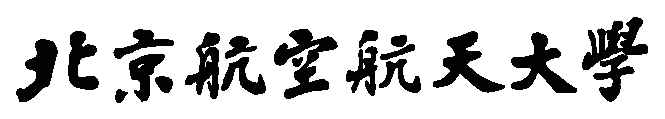
\includegraphics[width=.5\textwidth]{logo-buaa}
  \caption{测试图片\\第二行题注}
  \label{fig:logo}
\end{figure}
\centerline{-----------$\uparrow$-----------Space Check-----------$\uparrow$-----------}

我们在这儿插入一行字;

我们在这儿再插入一行字;

我们在这儿插入一行字;

我们在这儿再插入一行字;

我们在这儿插入一行字;

我们在这儿再插入一行字;

我们在这儿插入一行字;

我们在这儿再插入一行字;

\section{数学环境}

\subsection{数学符号}

模板定义了一些正体(upright)的数学符号:
\begin{center}
  \begin{tabular}{rl}
    \toprule
    符号                 & 命令 \\
    \midrule
    常数$\eu$     & \verb|\eu| \\
    复数单位$\iu$ & \verb|\iu| \\
    微分符号$\diff$ & \verb|\diff| \\
    $\argmax$         & \verb|\argmax| \\
    $\argmin$         & \verb|\argmin| \\
    \bottomrule
  \end{tabular}
\end{center}

更多的例子:
\begin{equation}
\eu^{\iu\pi} + 1 = 0
\end{equation}
\begin{equation}
\frac{\diff^2u}{\diff t^2} = \int f(x) \diff x
\end{equation}
\begin{equation}
\argmin_x f(x)
\end{equation}

\subsection{定理、引理和证明}

\begin{definition}
  If the integral of function $f$ is measurable and non-negative, we define
  its (extended) \textbf{Lebesgue integral} by
  \begin{equation}
  \int f = \sup_g \int g,
  \end{equation}
  where the supremum is taken over all measurable functions $g$ such that
  $0 \leq g \leq f$, and where $g$ is bounded and supported on a set of
  finite measure.
\end{definition}

\begin{example}
  Simple examples of functions on $\mathbf{R}^d$ that are integrable
  (or non-integrable) are given by
  \begin{equation}
  f_a(x) =
  \begin{cases}
  |x|^{-a} & \text{if } |x| \leq 1,\\
  0 & \text{if } x > 1.
  \end{cases}
  \end{equation}
  \begin{equation}
  F_a(x) = \frac{1}{1 + |x|^a}, \qquad \text{all } x \in \mathbf{R}^d.
  \end{equation}
  Then $f_a$ is integrable exactly when $a < d$, while $F_a$ is integrable
  exactly when $a > d$.
\end{example}

\begin{lemma}[Fatou]
  Suppose $\{f_n\}$ is a sequence of measurable functions with $f_n \geq 0$.
  If $\lim_{n \to \infty} f_n(x) = f(x)$ for a.e. $x$, then
  \begin{equation}
  \int f \leq \liminf_{n \to \infty} \int f_n.
  \end{equation}
\end{lemma}

\begin{remark}
  We do not exclude the cases $\int f = \infty$,
  or $\liminf_{n \to \infty} f_n = \infty$.
\end{remark}

\begin{corollary}
  Suppose $f$ is a non-negative measurable function, and $\{f_n\}$ a sequence
  of non-negative measurable functions with
  $f_n(x) \leq f(x)$ and $f_n(x) \to f(x)$ for almost every $x$. Then
  \begin{equation}
  \lim_{n \to \infty} \int f_n = \int f.
  \end{equation}
\end{corollary}

\begin{proposition}
  Suppose $f$ is integrable on $\mathbf{R}^d$. Then for every $\epsilon > 0$:
  \begin{enumerate}
    \renewcommand{\theenumi}{\roman{enumi}}
    \item There exists a set of finite measure $B$ (a ball, for example) such that
    \begin{equation}
    \int_{B^c} |f| < \epsilon.
    \end{equation}
    \item There is a $\delta > 0$ such that
    \begin{equation}
    \int_E |f| < \epsilon \qquad \text{whenever } m(E) < \delta.
    \end{equation}
  \end{enumerate}
\end{proposition}

\begin{theorem}
  Suppose $\{f_n\}$ is a sequence of measurable functions such that
  $f_n(x) \to f(x)$ a.e. $x$, as $n$ tends to infinity.
  If $|f_n(x)| \leq g(x)$, where $g$ is integrable, then
  \begin{equation}
  \int |f_n - f| \to 0 \qquad \text{as } n \to \infty,
  \end{equation}
  and consequently
  \begin{equation}
  \int f_n \to \int f \qquad \text{as } n \to \infty.
  \end{equation}
\end{theorem}

\begin{proof}
  Trivial.
\end{proof}



\subsection{自定义}

\newtheorem*{axiomofchoice}{Axiom of choice}
\begin{axiomofchoice}
  Suppose $E$ is a set and ${E_\alpha}$ is a collection of
  non-empty subsets of $E$. Then there is a function $\alpha
  \mapsto x_\alpha$ (a ``choice function'') such that
  \begin{equation}
  x_\alpha \in E_\alpha,\qquad \text{for all }\alpha.
  \end{equation}
\end{axiomofchoice}

\newtheorem{observation}{Observation}[chapter]
\begin{observation}
  Suppose a partially ordered set $P$ has the property
  that every chain has an upper bound in $P$. Then the
  set $P$ contains at least one maximal element.
\end{observation}
\begin{proof}[A concise proof]
  Obvious.
\end{proof}

\newtheorem{observationvar2}[observation]{Observationvar2}
\begin{observationvar2}
  Suppose a partially ordered set $P$ has the property
  that every chain has an upper bound in $P$. Then the
  set $P$ contains at least one maximal element.
\end{observationvar2}
\begin{proof}[A concise proof]
  Obvious.
\end{proof}

我们在这儿插入一行字;

我们在这儿再插入一行字;

我们在这儿插入一行字;

我们在这儿再插入一行字;

我们在这儿插入一行字;

我们在这儿再插入一行字;

我们在这儿插入一行字;

我们在这儿再插入一行字;

我们在这儿插入一行字;

我们在这儿再插入一行字;

我们在这儿插入一行字;

我们在这儿再插入一行字;

我们在这儿插入一行字;

我们在这儿再插入一行字;

我们在这儿插入一行字;

我们在这儿再插入一行字;

我们在这儿插入一行字;

我们在这儿再插入一行字;

% 总结
% !TeX root = ../Template.tex
% 总结
\summary
学位论文的结论单独作为一章,但不加章号。如果不可能导出应有的结论,也可以没有结论而进行必要的讨论。

\par * 嗯,这就是你的论文了 * \par


% 参考文献
% 2015版国标GBT7714-2015
% 2005版国标GBT7714-2005
\bibliographystyle{GBT7714-2015}
\bibliography{ref}

% 附录
% [附录]
\appendix

下列内容可以作为附录:

\begin{enumerate}[label=\arabic*)]
\item 为了整篇论文材料的完整,但编入正文又有损于编排的条理和逻辑性,这一材料包括比正文更为详尽的信息、研究方法和技术更深入的叙述,建议可以阅读的参考文献题录,对了解正文内容有用的补充信息等;
\item 由于篇幅过大或取材于复制品而不便于编入正文的材料;
\item 不便于编入正文的罕见的珍贵或需要特别保密的技术细节和详细方案(这中情况可单列成册);
\item 对一般读者并非必要阅读,但对专业同行有参考价值的资料;
\item 某些重要的原始数据、过长的数学推导、计算程序、框图、结构图、注释、统计表、计算机打印输出文件等。
\end{enumerate}

\par * 嗯,自由发挥吧 * \par

% 攻读学位期间成果
% [攻读学位期间取得的成果]
% \achievement = \chapter{攻读学位期间取得的成果}
\achievement

对于博士学位论文,本条目名称用“攻读博士学位期间取得的研究成果”,一般包括:

攻读博士学位期间取得的学术成果:攻读博士学位期间取得的学术成果:列出攻读博士期间发表(含录用)的与学位论文相关的学术论文、发表专利、著作、获奖项目等,书写格式与参考文献格式相同;

攻读博士期间参与的主要科研项目:列出攻读博士学位期间参与的与学位论文相关的主要科研项目,包括项目名称,项目来源,研制时间,本人承担的主要工作。

对于硕士学位论文,本条目名称用“攻读硕士学位期间取得的学术成果”,只列出攻读硕士学位期间发表(含录用)的与学位论文相关的学术论文、发表专利、著作、获奖项目等,书写格式与参考文献格式相同。

\par * 嗯,研究生不列科研项目 * \par

% 致谢
% [致谢]
\acknowledgments

致谢中主要感谢指导教师和在学术方面对论文的完成有直接贡献及重要帮助的团体和人士,以及感谢给予转载和引用权的资料、图片、文献、研究思想和设想的所有者。致谢中还可以感谢提供研究经费及实验装置的基金会或企业等单位和人士。致谢辞应谦虚诚恳,实事求是,切记浮夸与庸俗之词。

\par * 嗯,感谢完所有人之后,也请记得感谢一下自己 * \par

% 作者简介
% !TeX root = ../Template.tex
% [作者简介]
\biography
博士学位论文应该提供作者简介,主要包括:姓名、性别、出生年月日、民族、出生的;简要学历、工作经历(职务);以及攻读博士学位期间获得的其他奖项(除攻读学位期间取得的研究成果之外)。

\par * 嗯,“硕士学位论文无此项”,《手册》上是这么说的 * \par

\end{document}